\appendix

\subsubsection*{Auto-Start des Skripts beim Hochfahren des Raspberry Pi}
Um Programme oder Dienste automatisch bei Systemstart zu laden, gibt es die Möglichkeit, diese in die Datei \textbf{/etc/rc.local} einzutragen. Dazu muss man die Datei in einem Text-\\editor mit Root-Rechten öffnen und einen \textbf{vollständigen Pfad} zum auszuführenden Programm angeben. Wichtig ist, den Eintrag \textbf{vor} dem \textbf{\texttt{exit 0}} zu platzieren. \newline 
Zusätzlich wird durch Anhängen eines \textbf{\&} das Programm in den Hintergrund geschoben. Dies ist bei Vorhandensein einer Endlossschleife wichtig, da rc.local sonst nicht weiter abgearbeitet wird und der Raspberry Pi somit beim Starten hängen bleibt. \newline
Beim Testen der Funktionalität trat das Problem auf, dass das Skript sich nicht wie gewünscht verhält, wenn es sofort bei Systemstart aufgerufen wird. Das Programm ist zwar als laufender Prozess eingetragen, es werden jedoch keine Daten in die Datenbank geschrieben. Abhilfe schafft eine Verzögerung der Ausführung mit dem Befehl \textbf{\texttt{sleep}}.\newline
Die resultierende \textbf{rc.local}-Datei zeigt \autoref{lst:rc}

\lstinputlisting[label = lst:rc, caption=rc.local Datei]{lst/rc_local.txt}


\section{Serielle Schnittstelle zum Raspberry Pi}

Zur Nutzung der Schnittstelle muss diese zunächst im Konfigurationsmenü unter 'Advanced Options' eingeschaltet werden. Anschließend können die GPIO-Pins 4 und 5 als Tx bzw. Rx genutzt werden. Zum Testen der Funktionsfähigkeit wird die Software \texttt{minicom} genutzt. Durch den Befehl \texttt{sudo minicom -b 115200 -D /dev/ttyS0 -o} lässt sich die Schnittstelle öffnen. Pin 4 und Pin 5 werden mit einem Kabel verbunden und per \texttt{minicom} Zeichen gesendet. Diese erscheinen in der Konsole.



\section{FHEM-Modul für Plugwise-Steckdosen}
FHEM bietet ein internes Modul an, um die Steckdosen anzusprechen und zu konfigurieren. Um dieses zu benutzen,legt man ein neues device an (define myPlugwise Plugwise /dev/ttyUSB0). Dadurch wird der Stick definiert.


Die Abbildungen unten zeigen das FHEM-Menü und ausgelesene Daten (Energieverbrauch).\newline

\begin{figure}[H]
  \caption{FHEM Hauptseite}
  \centering
  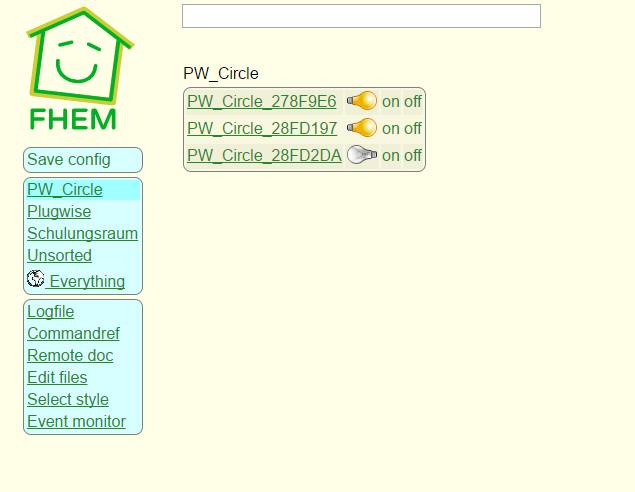
\includegraphics[width=6cm]{Home1}
\end{figure}

\begin{figure}[H]
  \caption{Konfigurationsmenü des Plugwise Sticks}
  \centering
  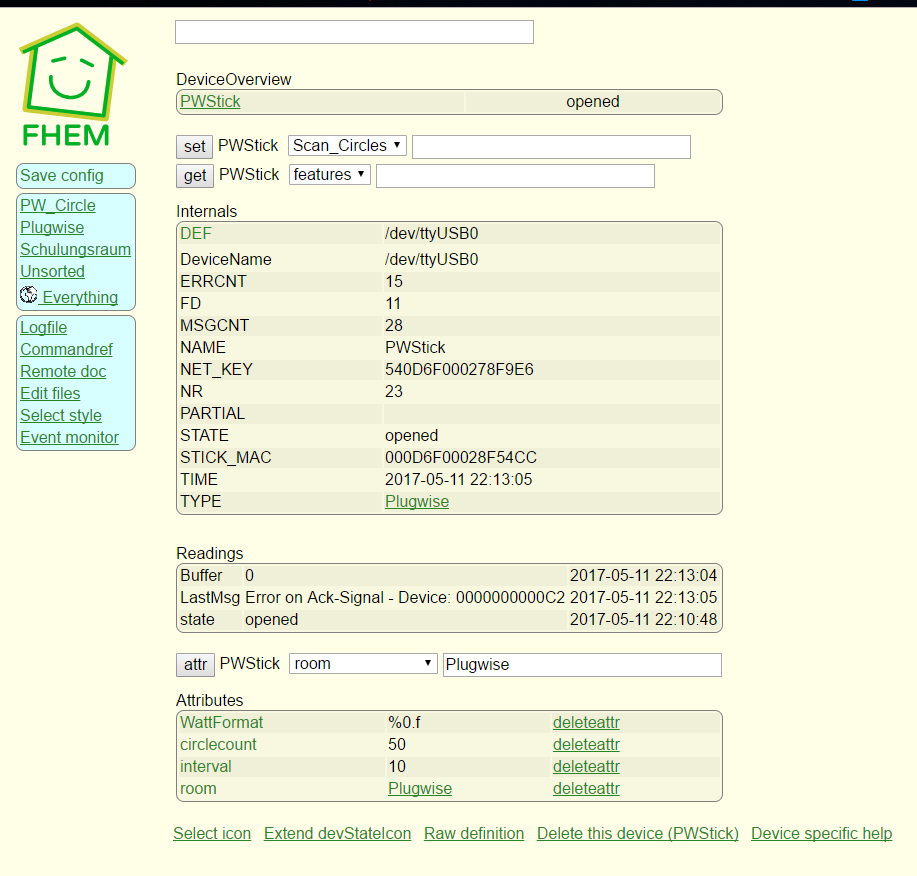
\includegraphics[width=6cm]{PWStick}
\end{figure}

\begin{figure}[H]
  \caption{Ausgelesener Energieverbrauch (Ausschnitt)}
  \centering
  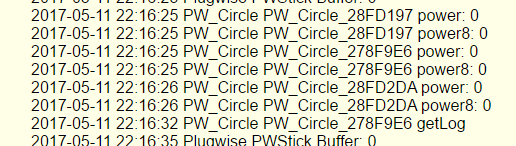
\includegraphics[width=0.5\textwidth]{FHEMPowerlogklein}
\end{figure}

\subparagraph{Probleme}\mbox{} \\
Damit die Circles überhaupt gefunden werden, muss versucht werden, parallel zu FHEM andersweitig die Steckdosen anzusprechen, z.B. mittels \texttt{plugwise-util}. Dabei findet FHEM nur einige der Steckdosen. Außerdem können nach einer Weile die Steckdosen nicht mehr gesteuert werden.\newline \newline

